\section{\crossflow Architecture and Design}
\label{sec:architecture}

In this section, we describe the architecture and design of \pmac. In Section~\ref{sec:mac}, we introduce the proposed MAC layer abstraction. Then, in Section~\ref{sec:topology}, we describe the topology in which the \pmac operates and in Section~\ref{sec:messages}, we describe how we extend the OpenFlow protocol to accommodate \pmac messages.


\begin{figure}[t]
  \centering
  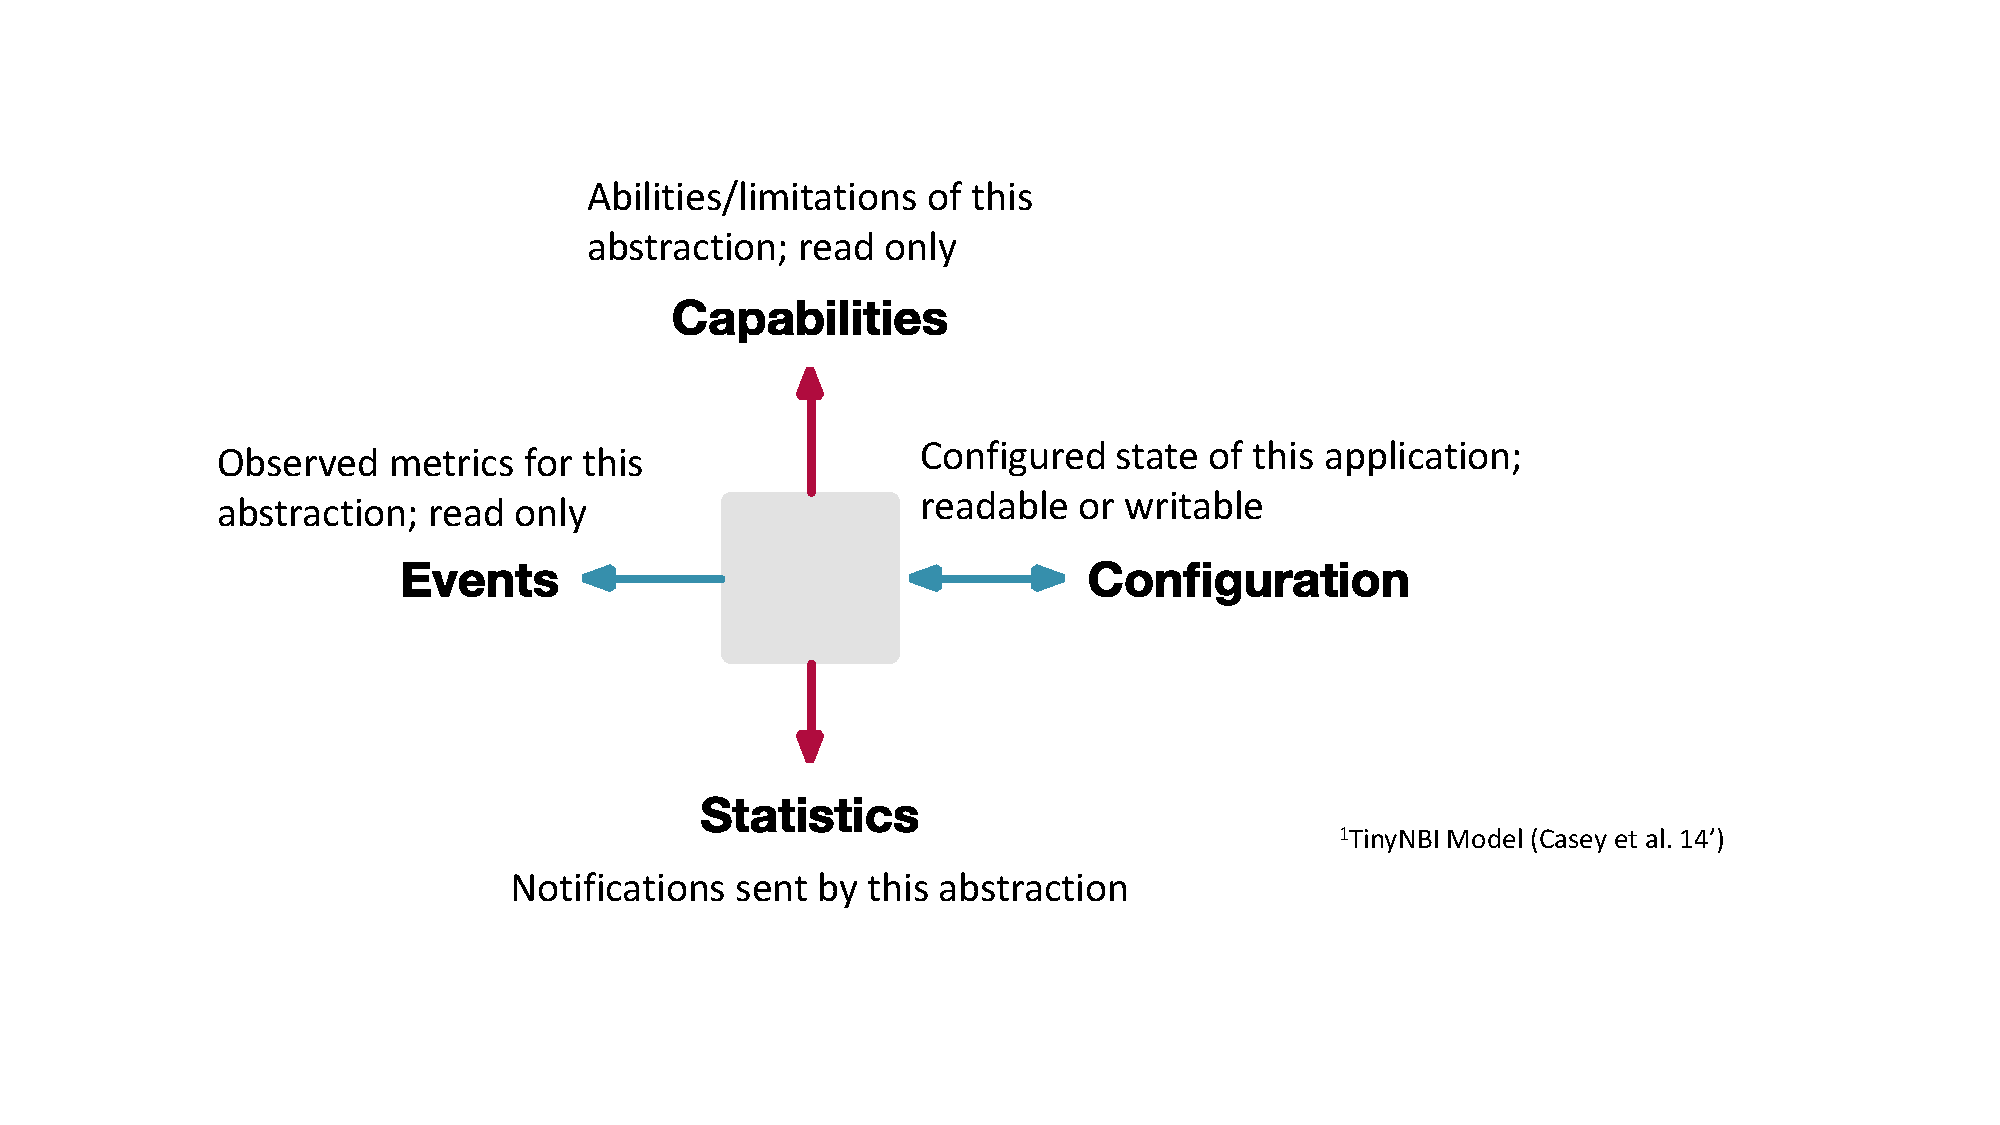
\includegraphics[width=0.6\textwidth]{figures/abstract.pdf}
  \caption{Interfaces exposed by an abstract entity}
  \label{fig:abstract}
\end{figure}

\begin{figure}[t]
  \centering
  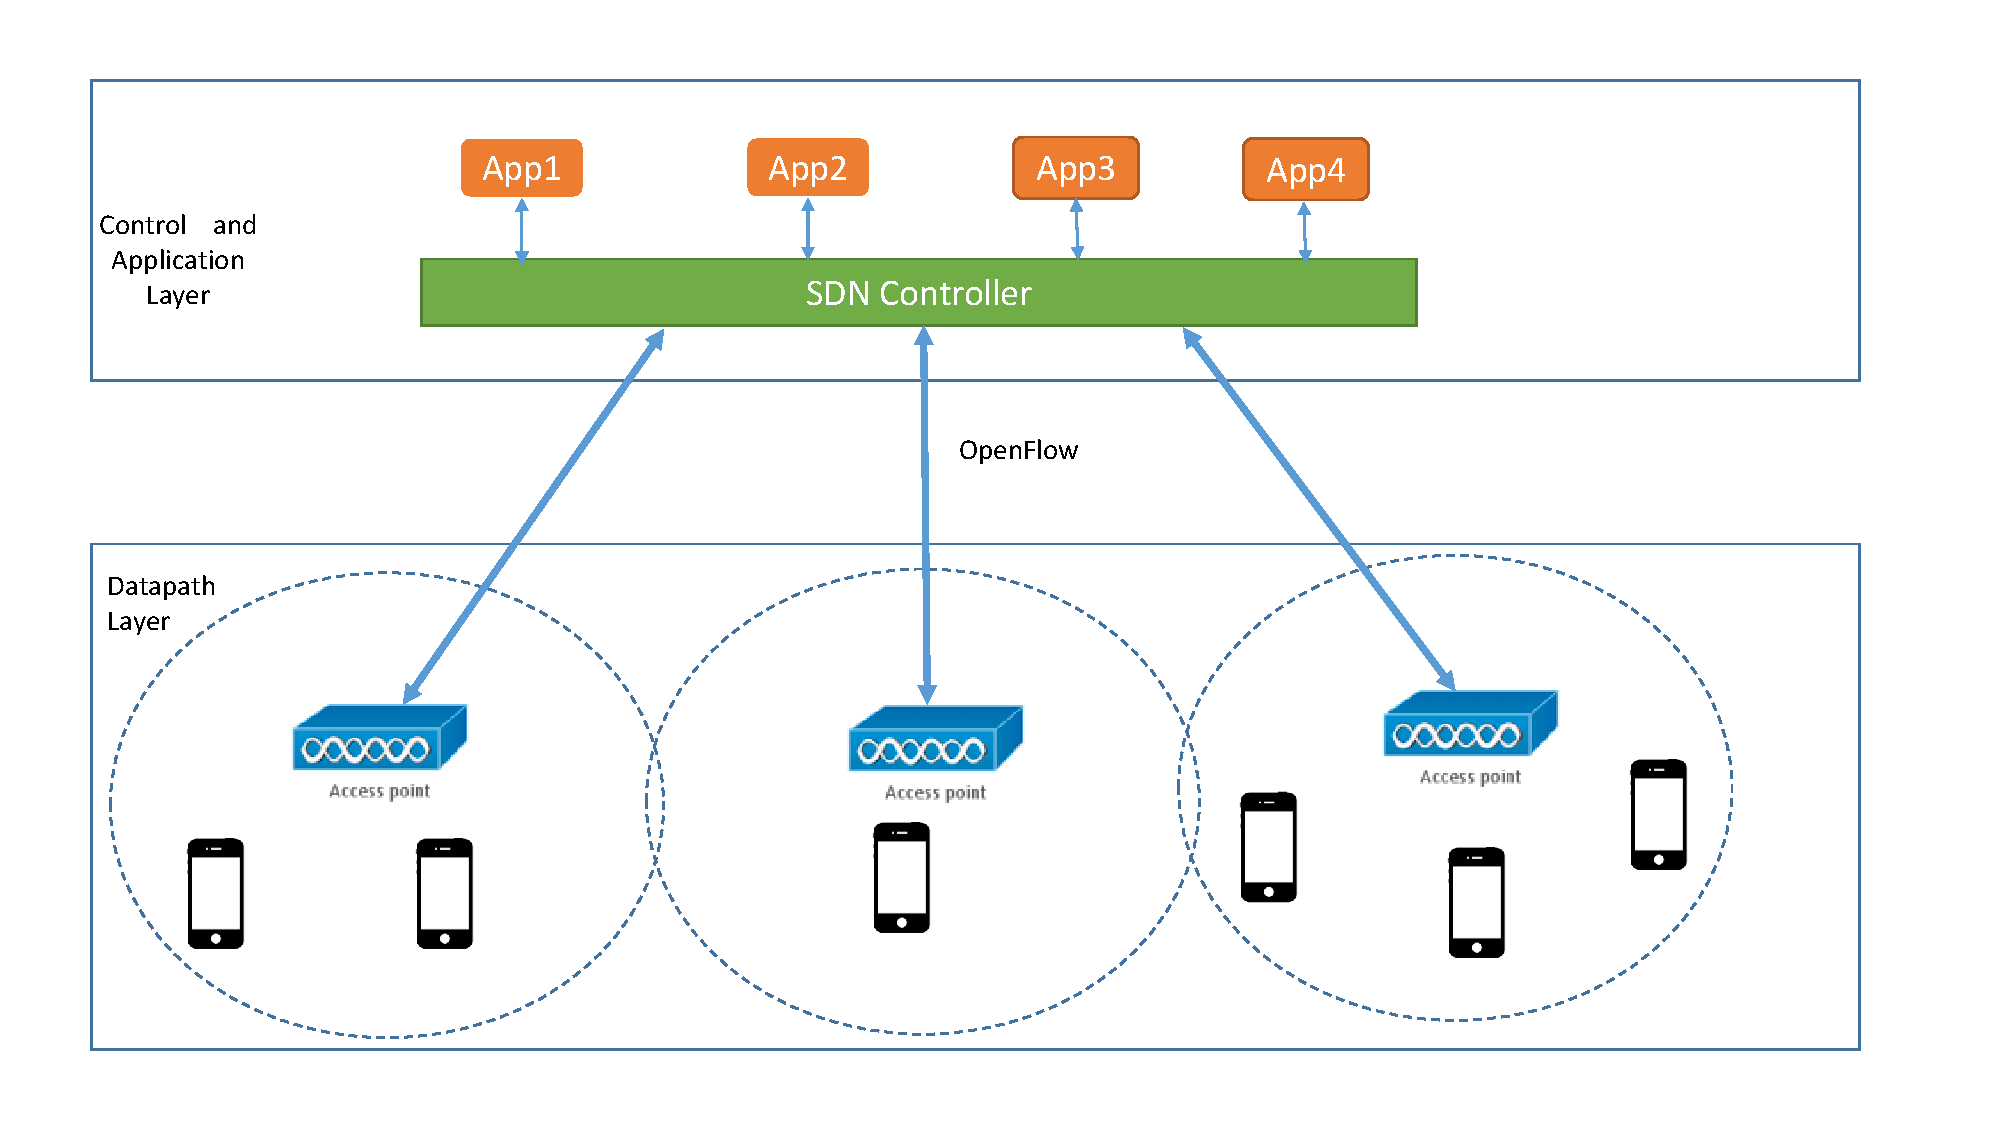
\includegraphics[width=0.6\textwidth]{figures/infrastructure.pdf}
  \caption{Infrastructure diagram of \pmac}
  \label{fig:infrastructure}
\end{figure}

\subsection{MAC Layer Abstraction}
\label{sec:mac}
We use the TinyNBI model described in \cite{Casey:14}, where each abstract component exposes these four types of interfaces: configuration, capability, statistics and events as shown in Figure~\ref{fig:abstract}. As mentioned in Section~\ref{sec:intro}, we take the interface definitions from \cite{macproc} and categorize them in the following manner:

\begin{itemize}
\item \textbf{Capabilities}: The interface allows the SDN controller to query the capabilities of MAC layer such as:
    (i) MAC protocol being used;
    (ii) Maximum frame length and
    (ii) Transmit power  
\item \textbf{Configuration}: The interface allows the SDN controller to configure the properties of MAC layer such as:
    (i) Setting backoff interval;
    (ii) Updating congestion window;
    (ii) Changing MAC protocol; and
    (iv) Setting timer value  
\item \textbf{Statistics}: The interface allows the SDN controller to query the statistics of MAC layer such as:
    (i) Queue length;
    (ii) Cuurent backoff interval and
    (ii) Number of frames received  
\item \textbf{Configuration}: The interface allows the SDN controller to register for events of MAC layer such as:
    (i) Collissions;
    (ii) Channel up/down;
    (ii) Queue overflow; and
    (iv) Timer expiry  
\end{itemize}

\begin{figure}[t]
  \centering
  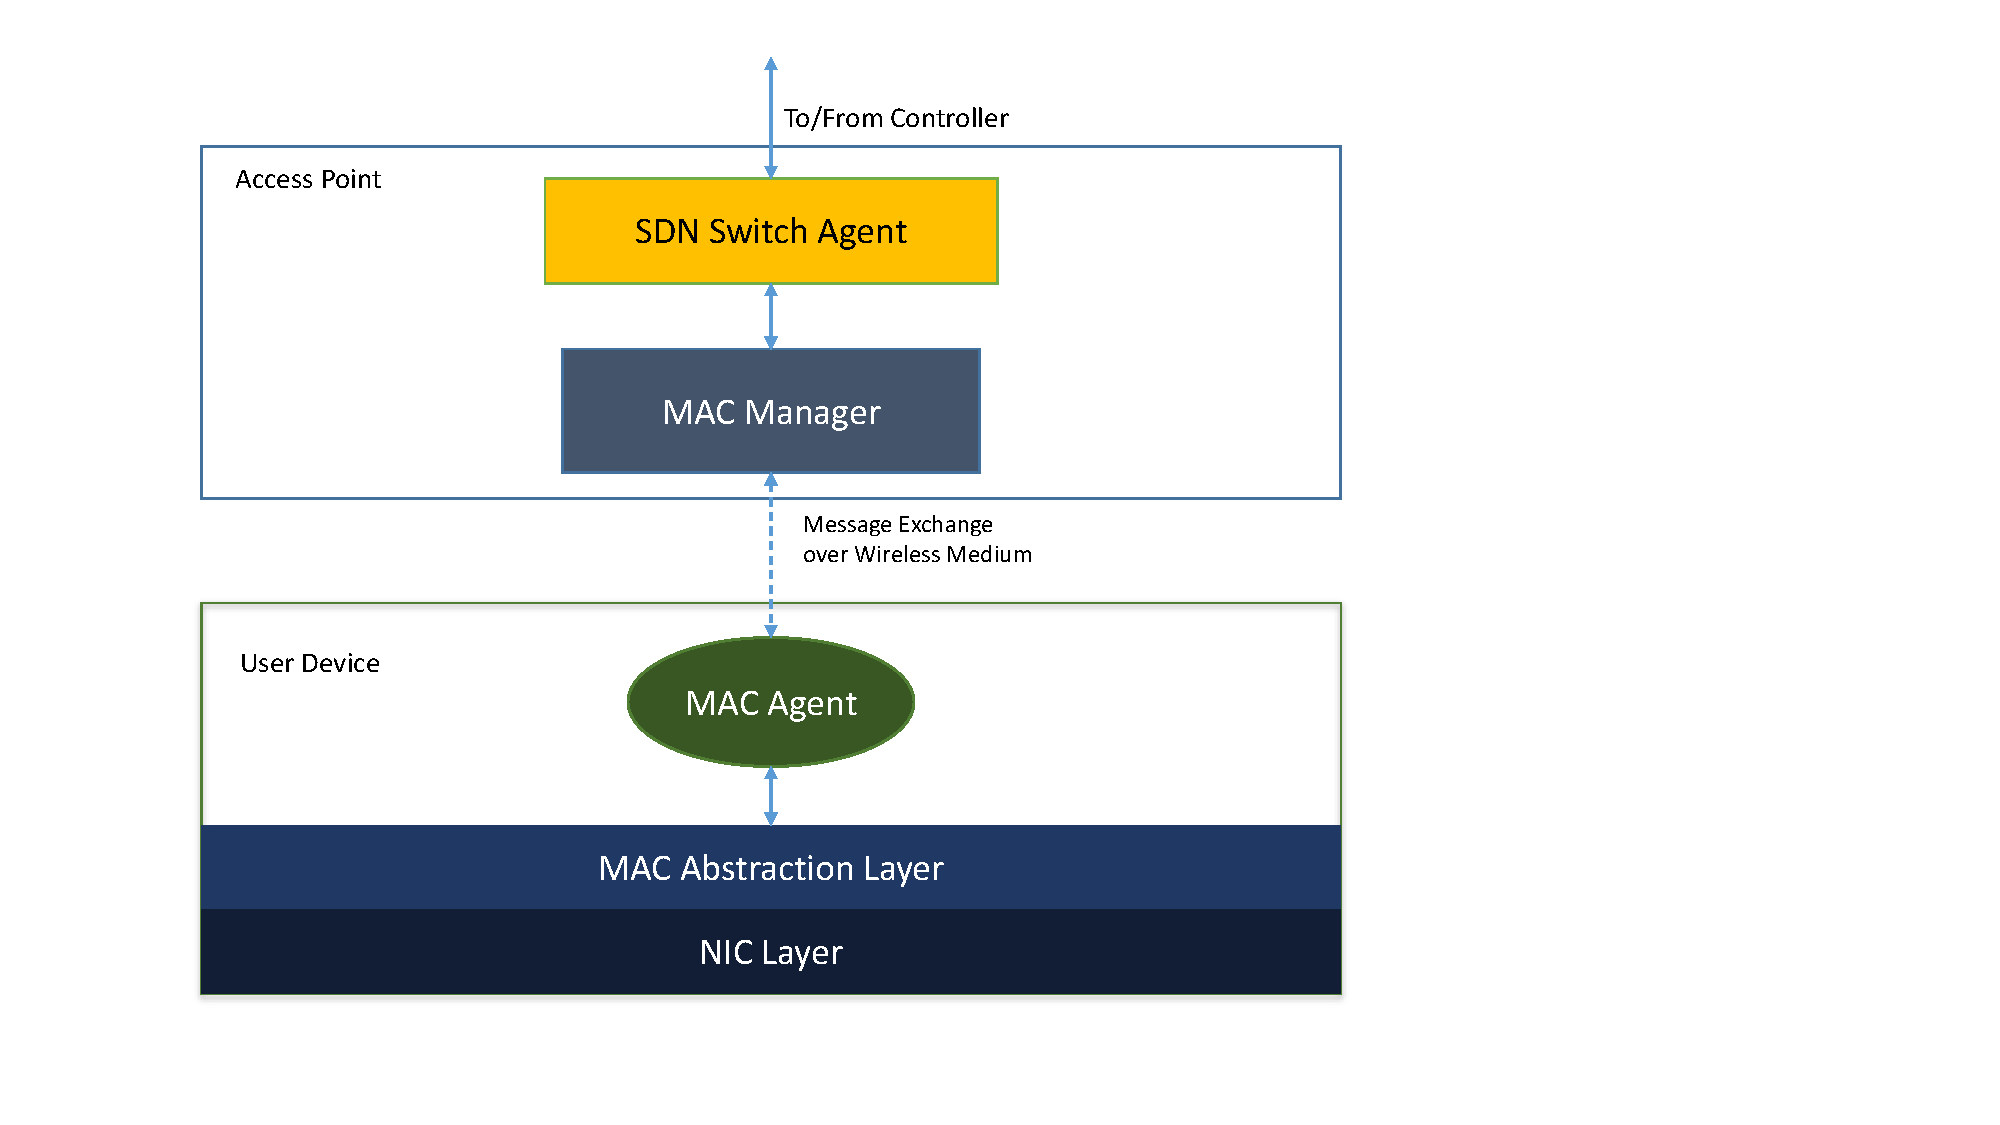
\includegraphics[width=0.6\textwidth]{figures/communication.pdf}
  \caption{MAC Manager (AP), MAC Agent and MAC abstraction layer(User devices) interaction}
  \label{fig:topology}
\end{figure}

\subsection{\pmac Topology}
\label{sec:topology}
In this paper, we consider the \pmac framework in a wireless network which operates in infrastructure mode as shown in Figure~\ref{fig:infrastructure}. The wireless clients are connected to the Access Points (AP), which are in turn, connected to a SDN controller. Each wireless client is composed of a MAC abstraction layer and a MAC agent running on top which is responsible for a MAC manager running in the AP. The MAC abstraction layer, on the other hand, is responsible for exposing the interface types as mentioned above. In a typical deployment scenario, the controller will send request to the AP, which is received by the MAC manager. The MAC manager then sends this requests to all the MAC agents running in the devices. This information can be piggybacked in beacon responses between devices and AP. On the response side, the MAC agents collect the information from the MAC abstraction layer and sends the information to MAC manager in AP through beacon requests. These responses are collected from all the devices associated with the AP, and an event report is sent to the controller. An illustrative diagram of this operation is shown in Figure~\ref{fig:topology}. 

\begin{figure}[t]
  \centering
  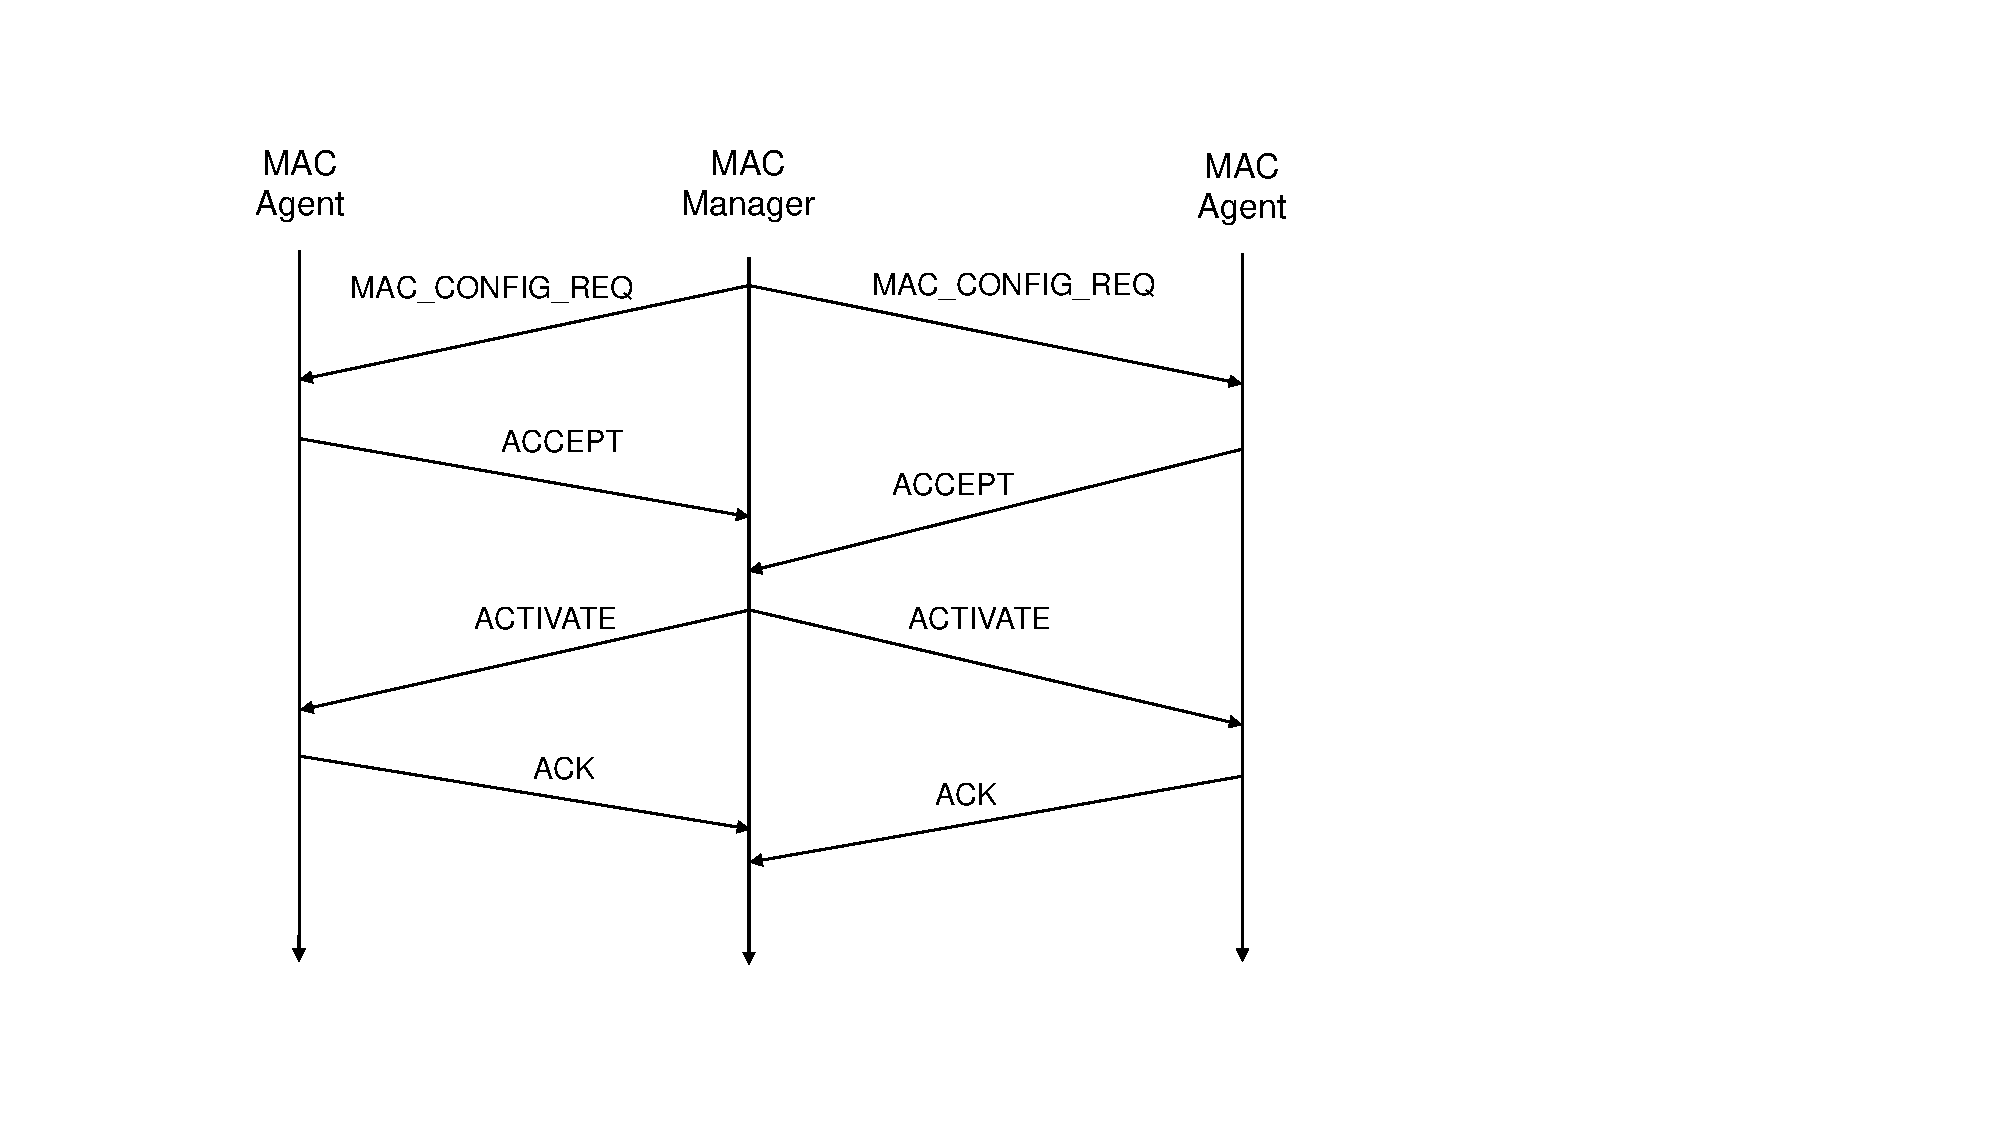
\includegraphics[width=0.6\textwidth]{figures/protocol.pdf}
  \caption{4-way handshake model between MAC Manager and MAC Agent for configuration messages in \pmac}
  \label{fig:protocol_feature}
\end{figure}

In order to support configuration messages, the \pmac framework needs to consider the synchronization issue which may arise due to inconsistencies  while applying the configuration. We developed a 4-way handshake protocol between the MAC manager and MAC agents so that configuration messages are applied in a reliable manner. As shown in Figure~\ref{fig:protocol_feature}, in the first step, the MAC Manager sends a \texttt{MAC-CONFIG-REQ} to all the MAC agents. Upon receiving this request, the agents communicate with the MAC abstraction layer to load the configuration and send  \texttt{ACCEPT} messages to the MAC Manager. Upon receiving all the \texttt{ACCEPT} messages, the MAC Manager sends \texttt{ACTIVATE} message to the agents to activate the configuration. Upon successful application of configuration, the agents send an \texttt{ACK} response and the MAC Manager informs the controller about the change of configuration. If any failure happens, similar process is used to rollback the configuration and a report is sent to the controller 

\subsection{Message Extensions}
\label{sec:messages}
  		  
\pmac uses SDN design principles to configure the MAC layer of devices thorough APs. As OpenFlow protocol does not natively support wireless MAC layer functionality, we extend the OpenFlow protocol to include such messages. For implementation purposes, we can use Experimenter fields of OpenFlow protocol which is used to define vendor specific information. We envision the following OpenFlow message extensions in \pmac:
\begin{itemize}
\item Capabilities message request - Request for the capability of MAC layer of devices like MAC protocl being used, frame length etc
\item Configuration message request - Request for modification of parameters like MAC protocol, timer value etc.
\item Statistics message request - Request for statistics such as queue length, current backoff interval etc.
\item Event message response - Response for events like collissions, timer expiry etc.
\end {itemize}
